\documentclass{deliverablereport}
\usepackage{wrapfig}
\usepackage{pdflscape}
\lstset{stringstyle=\tiny}

\deliverable{UI}{ipython-advanced-interacts}
\deliverydate{31/08/2018}
\duedate{31/08/2018 (M36)}
\author{Odile Bénassy and Nicolas M. Thiéry}

\begin{document}
\maketitle
% This will be the abstract, fetched from the github description
\githubissuedescription

\clearpage
\tableofcontents

\section{Introduction}

The \href{https://jupyter.org}{Jupyter Notebook} is a web application
that enables the creation and sharing of executable documents
containing live code, equations, visualizations and explanatory text.
Reaching far beyond the standard
\href{https://en.wikipedia.org/wiki/Read-eval-print_loop}{REPL}
interaction (Read-Eval-Print Loop), a key feature of Jupyter is its
\href{http://jupyter.org/widgets}{Interactive widgets} which enable
real time interactive data visualizations; the Jupyter community has
developed a large array of widgets for interactive 2D and 3D
visualization of data in the form of charts, maps, tables, etc;
See Figure~\ref{fig:ipyleaflet} for an example, and
\delivref{UI}{vis3d} for ODK's contribution to 3D visualization.
Furthermore, widgets can be \emph{composed} to build rich
applications, with all the usual UI components (e.g. menus, sliders,
or layout control); see Figure~\ref{fig:ipyleaflet2}.
%
Hence, the Jupyter stack provides a very flexible environment catering
for use cases ranging from a novice user typing just a few commands
or browsing interactive documents to more advanced users authoring
rich interactive applications for their fellows.

\begin{figure}[h]
  \begin{center}
    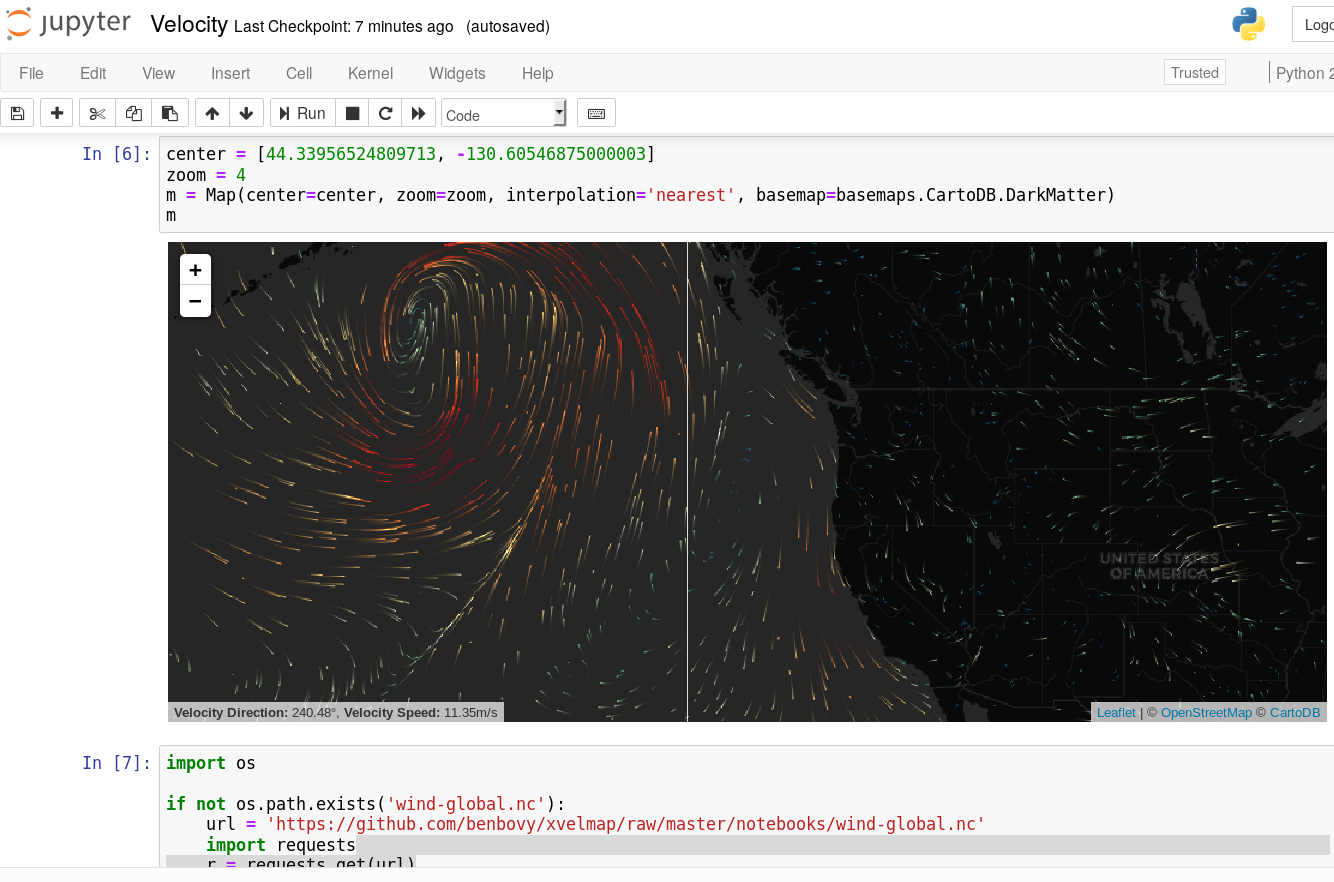
\includegraphics[width=\textwidth]{images/Velocity}
  \caption{A Jupyter widget displaying an interactive map based on
  OpenStreetMap data, overlayed with a visualisation of wind velocity
  data \tiny{(courtesy of the \lstinline{ipyleaflet} documentation)}.}
  \label{fig:ipyleaflet}
  \end{center}
\end{figure}

\begin{figure}[h]
  \begin{center}
    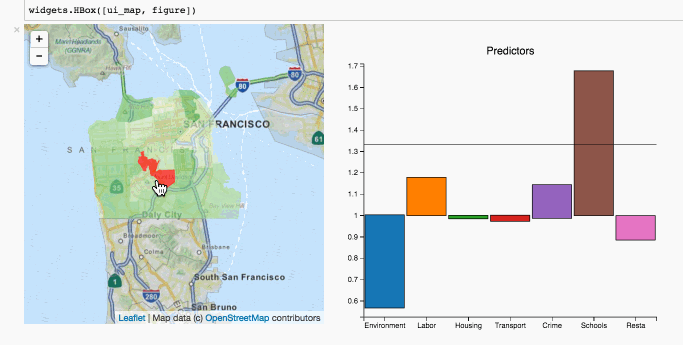
\includegraphics[width=\textwidth]{images/sc-ipyleaflet}
    \caption{A Jupyter application displaying survey results on San
      Francisco city districts \tiny{(courtesy of the \lstinline{ipyleaflet} documentation)}.}
  \label{fig:ipyleaflet2}
  \end{center}
\end{figure}

The question we are tackling in this report is how this technology --
and specifically Jupyter widgets -- can be leveraged for pure
mathematics. The unique challenge comes from the huge variety of
mathematical objects that the user may want to visualize and
interact with, and the variety of graphical representations;
see Figure~\ref{fig:math_viz} for some examples.
%
We therefore can't hope to provide hand crafted solutions for each
situation; instead we need to devise a toolbox of generic solutions
from which users can easily derive specialized visualizations for
their own pet objects.

%\newpage

\begin{figure}%[h]
  \begin{center}
    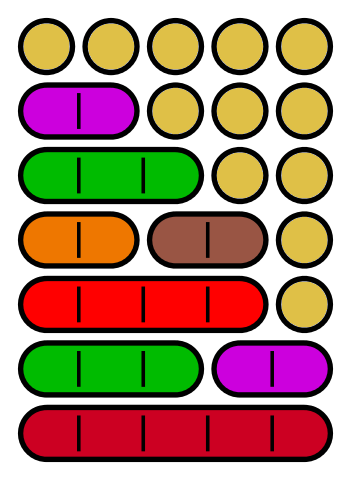
\includegraphics[width=0.20\textwidth]{images/partitions-of-5}
    \hfil\hfil
    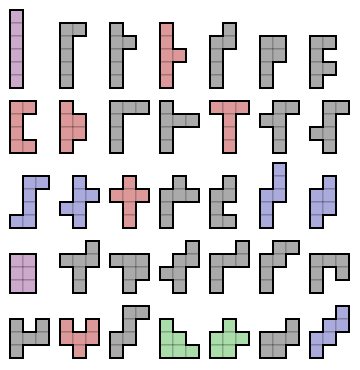
\includegraphics[width=0.25\textwidth]{images/hexominoes}
    \hfil
    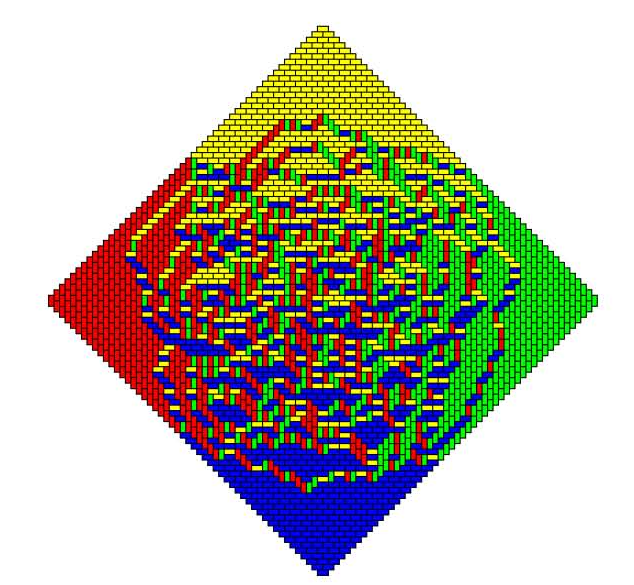
\includegraphics[width=0.30\textwidth]{images/AztecDiamond}
%   \end{center}
% \end{figure}
% \begin{figure}[h]
%   \begin{center}
    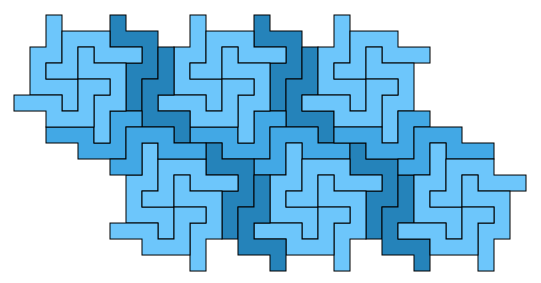
\includegraphics[width=0.4\textwidth]{images/nonominoes}
    \hfil
    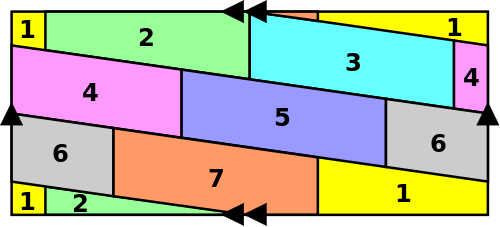
\includegraphics[width=0.4\textwidth]{images/500px-Torus_with_seven_colours}
%   \end{center}
% \end{figure}
% \begin{figure}[h]
%   \begin{center}
    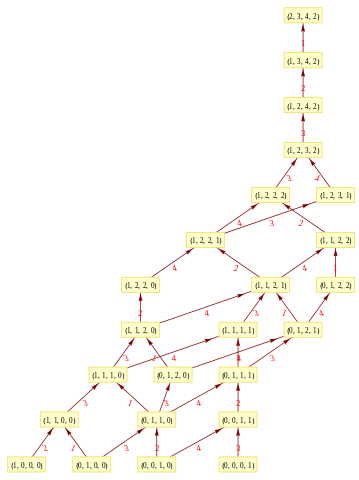
\includegraphics[width=0.3\textwidth]{images/359px-F4HassePoset}
    \hfil
    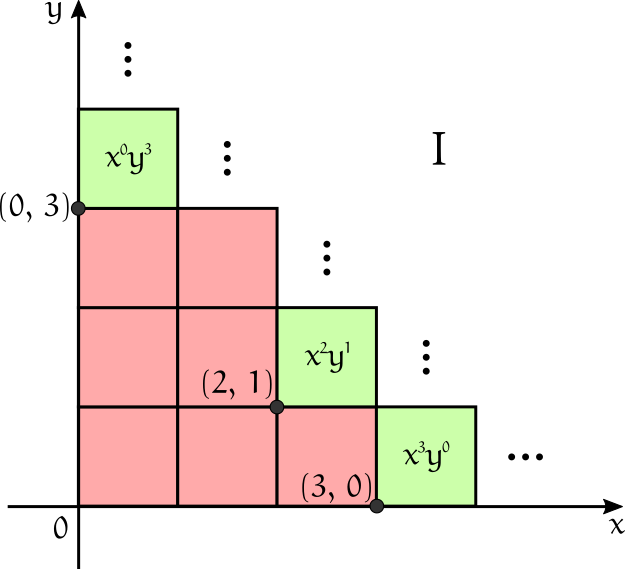
\includegraphics[width=0.3\textwidth]{images/Wikipic}
    \hfil
    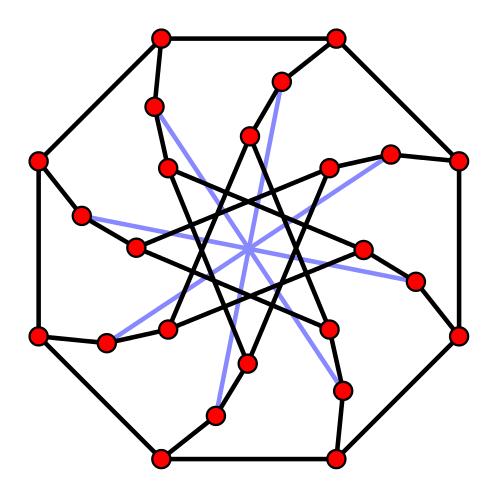
\includegraphics[width=0.3\textwidth]{images/500px-McGee_graph}
%   \end{center}
% \end{figure}
% \begin{figure}[h]
%   \begin{center}
    
\includegraphics[width=0.3\textwidth]{images/fractioncont}
    \hfil
    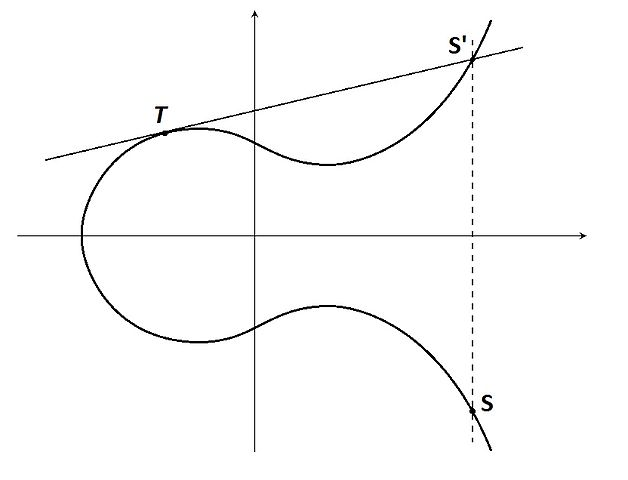
\includegraphics[width=0.3\textwidth]{images/elliptic-curve}
    \hfil
    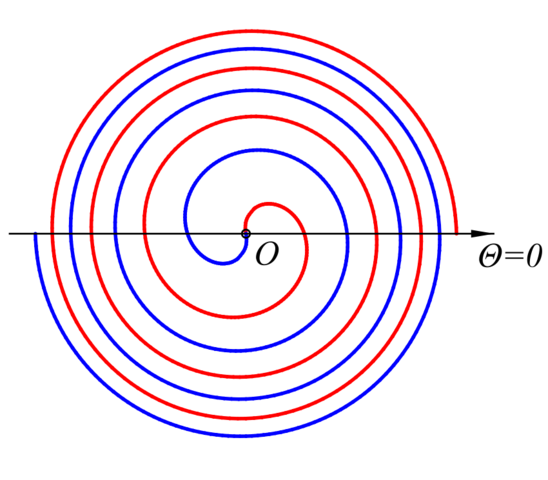
\includegraphics[width=0.3\textwidth]{images/548px-Fermat's_spiral_01}
%   \end{center}
% \end{figure}
% \begin{figure}[h]
%   \begin{center}
    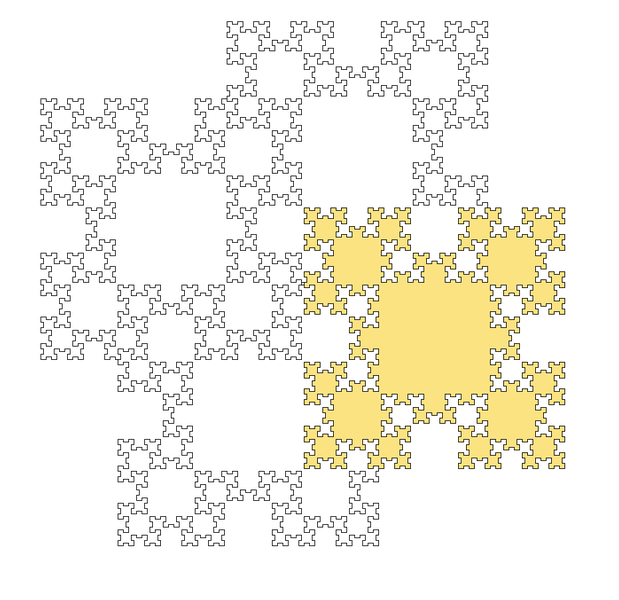
\includegraphics[width=0.3\textwidth]{images/619px-Tiling_Fibonacci_word_fractal}
    \hfil
    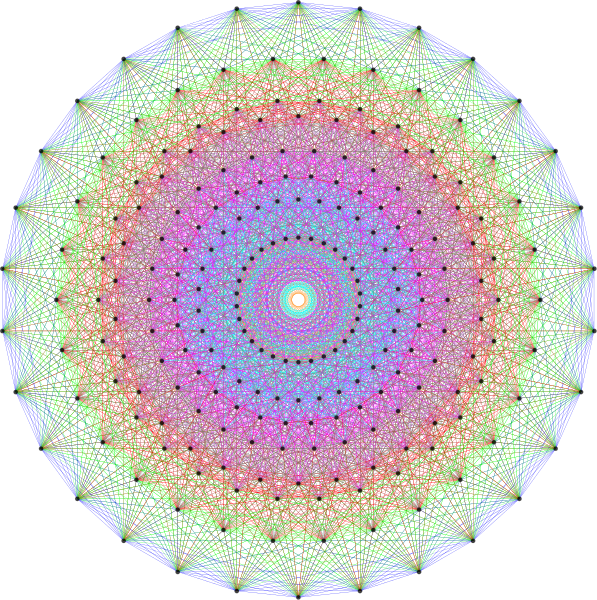
\includegraphics[width=0.3\textwidth]{images/597px-E8Petrie}
  \end{center}
  \caption{Some graphical visualizations of mathematical objects}
  \label{fig:math_viz}
\end{figure}

We pursue two directions:

In Section~\ref{section:combi}, we explore the development of widgets
for the graphical visualization in combinatorics -- or more generally
discrete mathematics. The choice of this area of mathematics was, to
some extent out of personal interest and expertise, but more
importantly because devising good representations -- mental images --
of discrete objects is at the heart of research in combinatorics. We
start by reviewing in Section~\ref{section:francy} the GAP package
\href{https://github.com/mcmartins/francy}{Francy} which currently
explores the natural use case of objects that admit a graph-like
representation: trees, graphs, lattices of subgroups, crystals,
posets, discrete markov chains, just to name a few. At this stage, ODK
has a light contribution to the development of this package, through
the supervision of \ODK's member Markus Pfeiffer. We highlight the
lessons learned there and describe upcoming collaboration toward
bringing Francy\'s features to SageMath.

Then, in Section~\ref{section:grid}, we report on the implementation
in SageMath of a generic widget for objects that admit a
representation as a collection of cells on a 2D grid, and
specializations for typical objects such as partitions, tableaux,
polyominos, aztec diamonds, mazes. One aspect which we explore beyond
Francy is not only \emph{interactive visualization} but also
\emph{interactive edition}, where the underlying mathematical object
gets changed by the user gestures. This is the occasion to explore the
flexibility of the the design patterns emerging from Francy.

The choice of this use case was motivated by two important features:
\begin{itemize}
\item the visualization part is relatively simple making it a good
  case for prototyping;
\item the potential impact is high due to the large number of objects
  covered, bringing in opportunities for testing how users manage to
  to adapt our generic tools for their own pet objects;
\end{itemize}

In a second direction, we explore in
Section~\ref{section:sage-explorer} the use of Jupyter widgets not only
for the graphical visualization of an object, but for displaying a
page offering a synthetic overview of the information about that
object, including type, important properties and invariants, available
operations, related objects, documentation, etc. All sort of
information that is readily available by introspection but that a UI
can make easy to discover and emphasize according to relevance. The
challenge is that, given the huge variety of objects in a system like
SageMath, we can't afford to hand craft such pages for each type of
objects. We report on our prototype
Sage-Explore that exploits the semantic embedded into the
system to produce a reasonable overview page automatically tailored to
each object.

%\TODO{Screenshot of Sage-explorer?}
% here is one, on the usual StandardTableau(15)
% I can try to make more, but at least the PetersenGraph fails (the
% cell is much too small for seing anything)

\begin{figure}[h]
  \begin{center}
    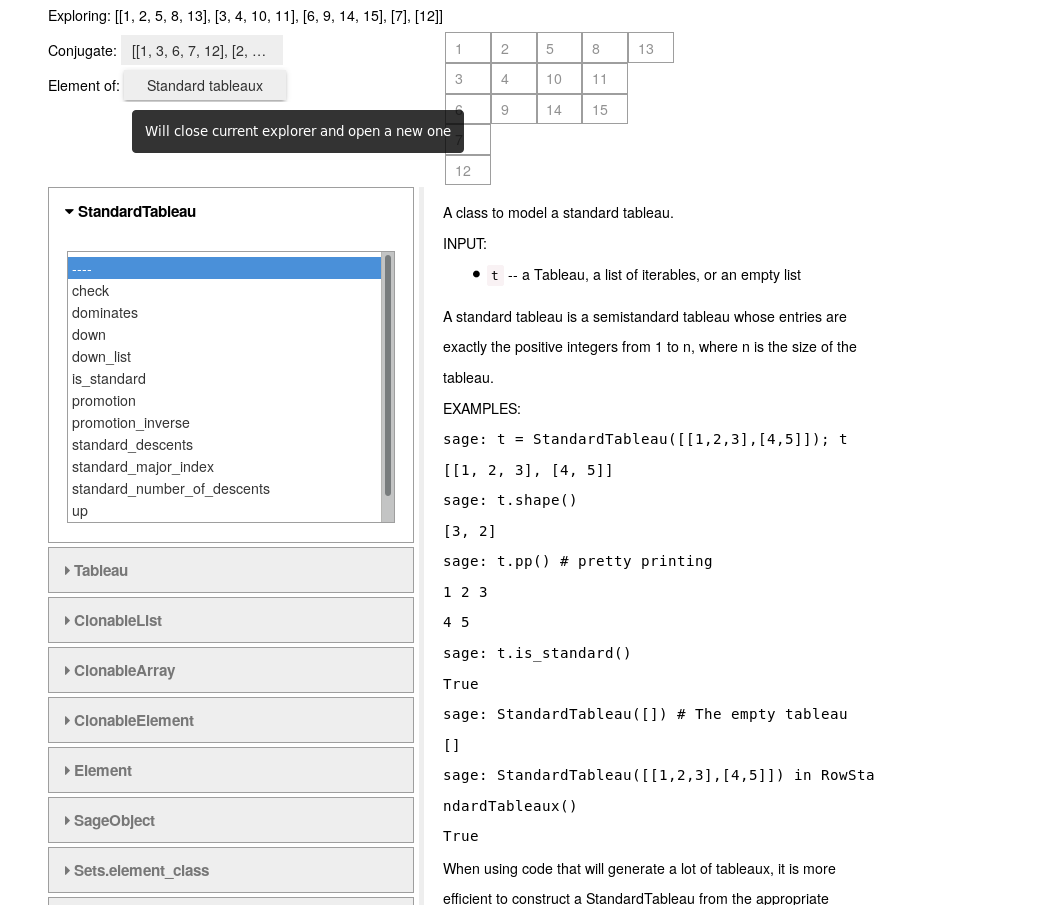
\includegraphics[width=\textwidth]{images/TableauExplorer}
  \end{center}
  \caption{Interactive introspection on a standard tableau with Sage-Explorer}
  \label{fig:tableau-explorer}
\end{figure}


Altogether, the Jupyter Widget technology has proven as mature and
flexible as we hoped for. Designing new widgets does take some
expertise, but from the experience we gained, we are confident that it
lends itself well to the implementation of generic widgets by power
users that can be specialized by casual users and used by novices.

Three main challenges arise along the way which we will continue to
explore and tackle during the last year of OpenDreamKit:
\begin{itemize}
\item Implementing visualization widgets is time consuming and
  requires specific expertise that developers of computer algebra
  systems usually don't have. It's therefore desirable to reuse them
  across mathematical objects that share a certain type of
  visualization, and across computer algebra systems. How to best
  design widgets to decouple them from the specific objects or
  programming language at hand?
\item User interface and visualization technologies tend to evolve
  much faster than computational systems; how to best design widgets
  to decouple the semantic part of the visualization of the widgets
  from the actual visualization technology, in order to prepare for a
  smooth and cheap migration path when such technology evolves and
  foster long term sustainability?
\item Widgets, as all modern web technologies, rely a lot on
  asynchronous execution. This is quite a different model from the
  Read-Eval-Print main loop that many not-so-young computational
  systems (including SageMath!) have originally been designed for, and
  such systems don't always behave well under asynchronous pressure:
  we have faced some bad crashes. How deep is the difficulty? How hard
  will it be to resolve it?
\end{itemize}

% \TODO{tension SAGE/javascript concernant l'emplacement des appels de
%   méthodes}

\section{Interactive visualization of combinatorial objects}
\label{section:combi}

\subsection{Francy: an Interactive Discrete Mathematics Framework for GAP}
\label{section:francy}

Francy is a package for interactive visualisation in discrete
mathematics. It's developed mainly by Manuel Martins, with supervision
by ODK's member Markus Pfeiffer. For now, Francy has been focusing on
the interactive visualisation of objects that admit a graph-like
representation (trees, graphs, ...). Features include for example
zoom-and-pan, moving nodes, clustering, menus for
activating/deactivating interactions, etc. Those are basic interactive
graph drawing features and are not particularly impressive by
themselves: after all, interactive graph drawing and editing has been
the subject of a whole community, with series of conferences such as
the \emph{International Symposium on Graph Drawing and Network
  Visualization}, and acclaimed tools like \lstinline{graphviz} or
\lstinline{tulip}. What makes Francy stand is to bring those feature
to computational systems and, more importantly, explore how to best
leverage the technology to empower users of such systems to adapt it
to their needs.

At this stage, Francy is a package for the GAP computer algebra
system. However its features would be extremely valuable for other
systems and in particular \Sage. Also Francy uses Jupyter Widgets as
GUI framework and \href{d3js.org}{D3JS javascript library} library for
visualisation. %which manipulates the browser DOM for the graphical display itself
While those are flourishing technologies that are promising for the
years to come, lessons learned the hard way from the past (e.g. within
the xgap project) shows that, at the scale of decades, GUI and
visualization frameworks change at a faster pace than computational
systems and visualization needs.

To tackle these two tensions, Francy has taken the approach of
decoupling itself from the computational system and from the GUI
framework and visualization libraries. It does this by introducing an
intermediate layer of semantic models of what graphical
representations are. With this approach, integrating a new
computational system reduces to providing a backend describing the
desired graphical representations for its mathematical objects in the
semantic model. Similarly, integrating GUI framework reduces to
providing a frontend describing how to concretely render and interact
with the graphical representations from the model. In practice, the
semantic model takes the form of an intermediate JSON data format,
with JSON data being passed from the computational system to the
browser.

\begin{figure}[h]
  \begin{center}
    
\includegraphics[width=\textwidth]{schemas/SensUnique}
  \end{center}
  \caption{Interactive visualization Data Flow}
  \label{fig:dataflow1}
\end{figure}


%\subsection{Francy, }


\subsection{Toward interactive edition}
\label{section:editing}

We have seen a \emph{design pattern} emerging in the previous section:
without this being formalized, a similar approach had been taken in
Sage for static graph drawing, using the so-called ``dot'' format of
the graphviz project as intermediate data format, to later produce
graph pictures in a variety of formats (latex, pdf, svg).

\begin{wrapfigure}{r}{0.25\textwidth}
  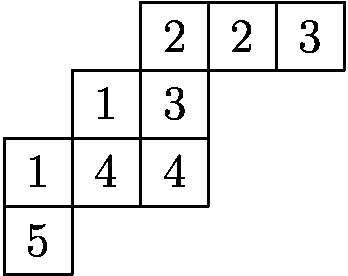
\includegraphics[width=100px]{images/JDTSlide}
  \caption{A skew-tableau}
  \label{fig:skew_tableau}
\end{wrapfigure}
Similarly, in the
\href{http://mupad-combinat.sourceforge.net}{MuPAD-Combinat} project a
generic intermediate data format was designed for all objects that can
be drawn by filling out certain cells in a 2-dimensional grid. For
example Figure~\ref{fig:skew_tableau} shows a drawing of \emph{skew
  tableau}, an important kind of combinatorial object arising in
representation theory.
We will call such a drawing a \emph{grid-like representation}.


From the intermediate data format, drawings could be produced in a
variety of format: latex, pdf, various forms of ascii art, \dots; see
\href{http://mupad-combinat.sourceforge.net/doc/en/Cat_Combinat/CombinatorialClassWith2DBoxedRepresentation.html}{Combinatorial Class With 2DBoxedRepresentation}.
This achieved the same two levels of decoupling as we have seen in Francy.

We decided to build on this previous experience to explore not only
visualization, but also \emph{interactive editing}: here, the interaction
not only affects the visualization, but also induces changes to the
the original mathematical objects via the intermediate data format.
Thus the data flow is now bidirectional.

\begin{figure}[h]
  \begin{center}
    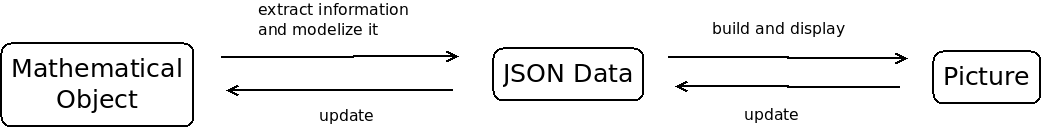
\includegraphics[width=\textwidth]{schemas/DoubleSens}
  \end{center}
  \caption{Interactive edition Data Flow}
  \label{fig:dataflow2}
\end{figure}

This brings new challenges.
%
% Please notice an additional challenge here: while editing cells or
% adding/removing them, the editor has to \emph{reconstruct} a new
% object from its cells and this requires also \emph{checking} the type of this
% potential new object and displaying messages during the editing
% process, especially in case of a temporary invalidity.

First, updates may fail: given that the intermediate data format does not
carry all the semantic of the mathematical objects, some interactive
editions may be invalid; yet such editions should not be necessarily
be forbidden, as it may take several elementary edition step to move
from one valid state to another (think of a text editor that would
block typing any key leading to a temporarily incorrectly spelled word!). Hence
some logic is needed to handle loss and recovery of sync between the
state of the semantic representation model and that of the
underlying mathematical object.

In addition, rich editing features, requires richer message passing
than just sending description of the object back and forth. For
example, in order to provide visual hints to the user, the view may
need to request what are the next valid edition steps for a given
object; or in case an invalid step is taken, the object may return
rich error messages enabling visual feedback. Also, for editing large
objects, one may wish as well to send only incremental updates.

Therefore, the semantic representation model needs not only to specify
a \emph{data format} to represent instances of this model, but also
\emph{operations} on them, that is an API.


Aiming for interactive editing was suggested by the Larch Environment.
In his \href{https://core.ac.uk/download/pdf/9839511.pdf}{master
  thesis} (2013), Geoffrey W. French presents his own graphical
interactive programming environment called \emph{larch}. One of his
main ideas is to \emph{coerce} objects into graphical representations,
meaning that every object must know how it can be graphically
represented. Moreover, this representation is only a default one and can be
tailored by the user: G.W. French speaks of different
\emph{perspectives} for the same object. The Larch Environment also
maintained a state of objects in order to automatically refresh the
representation. This project was meant as an experimental platform,
without a strong and widely used underlying infrastructure as \Jupyter,
and was discontinued in 2014. Nevertheless the
\href{https://www.youtube.com/watch?v=BaqaIw2c91o&t=29s}{online videos}
remain inspiring.
% However, the Larch environment was designed to run
% locally, i.e. not within any browser, and

\subsection{A generic widget for objects with a grid-like representation}
\label{section:grid}

To explore interactive editing, we set as goal the implementation of a
generic Jupyter widget meant for all \Sage-objects admitting a
grid-like representation.

This use case combined several advantages:
\begin{itemize}
\item The UI part was relatively straightforward, for example
  requiring no Javascript side extension;
\item Little mathematical background was required; this, together with
  the previous point, made for a smooth learning curve for our
  Research Software Engineer;
\item It was a low hanging fruit with a large coverage in algebraic
  combinatorics, including matrices, integer partitions, (standard)
  (skew) tableaux, ribbons, ribbon tableaux, grid graphs, aztec
  diagrams, etc.
\item The end result is immediately useful to colleagues, enabling
  early feedback from users;
\item There is a large variety of potential specializations, each with
  it's own quirks and specifics.
\end{itemize}
Hence, this use case provided a unique challenge: all the difficulty
resided in the the design of a generic editing solution that encapsulates as
much of the technicalities as possible, enabling users to specialize
the generic solution for their own pet objects with little expertise.

\subsection{Overview of the features and design}

The developed \Jupyter widget \emph{GridViewWidget} has the following
features:
\begin{itemize}
\item editing the content of cells
\item adding or removing cells
\item selecting cells for more interactions
\item supporting temporarily invalid states
\item recovering the underlying mathematical object for further
  computations.
\end{itemize}

\begin{wrapfigure}{r}{0.32\textwidth}
  \begin{center}
    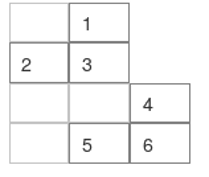
\includegraphics[width=.20\textwidth]{images/SkewTableauWidget}
    \qquad
    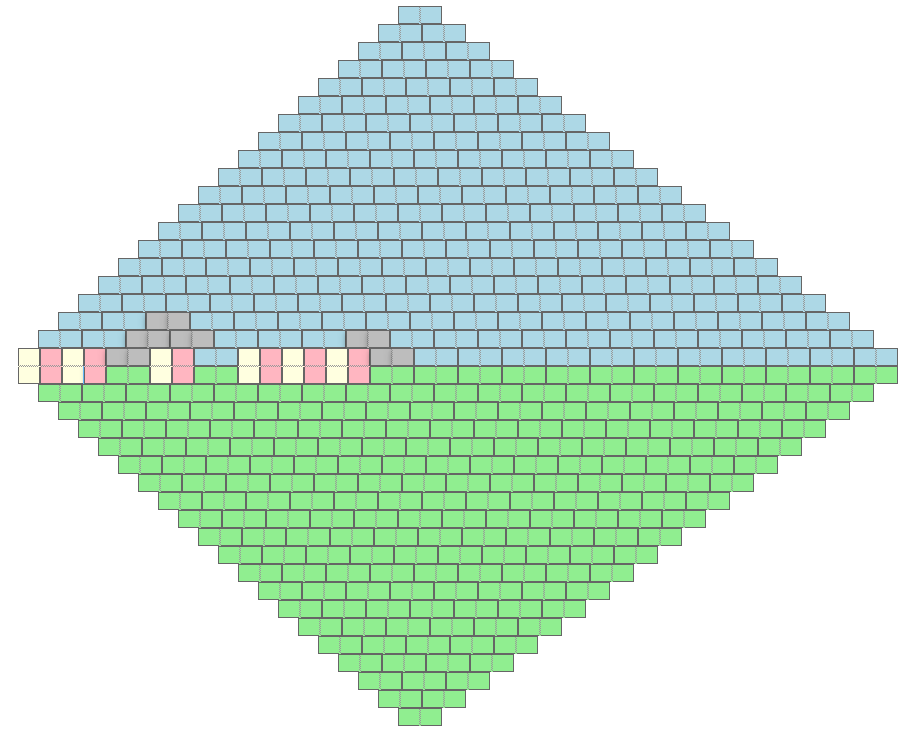
\includegraphics[width=.30\textwidth]{images/dominos-azteque}
  \end{center}
  \caption{Editing a skew tableau, and flipping dominos on a grid graph}
\end{wrapfigure}

The semantic representation model takes the form of a Python class
\emph{GridViewEditor} that is both agnostic of the GUI and of the
mathematical objects. To enable the latter, the interaction with
mathematical objects of a certain kind, say integer partitions, goes
through an adapter class which implements the required API on top of
that of integer partitions. See the Figure~\ref{fig:schema}.

The implementation of such an adapter shall be as simple as possible,
to empower users to write new ones for their own pet mathematical
objects. In particular, it should only require knowledge about the
business logic of ditto mathematical objects. We explored different
options, and battlefield tested them by writing adapters for a
selection of mathematical objects of different nature, chosen in
collaboration with potential users at the occasion of the experimental
mathematics Spring school MathExp 2018 coorganised by \ODK
(see~\longdelivref{dissem}{workshops-3}). The final design will be
chosen according to users feedback.

\begin{landscape}
\begin{figure}[h]
  \begin{center}
    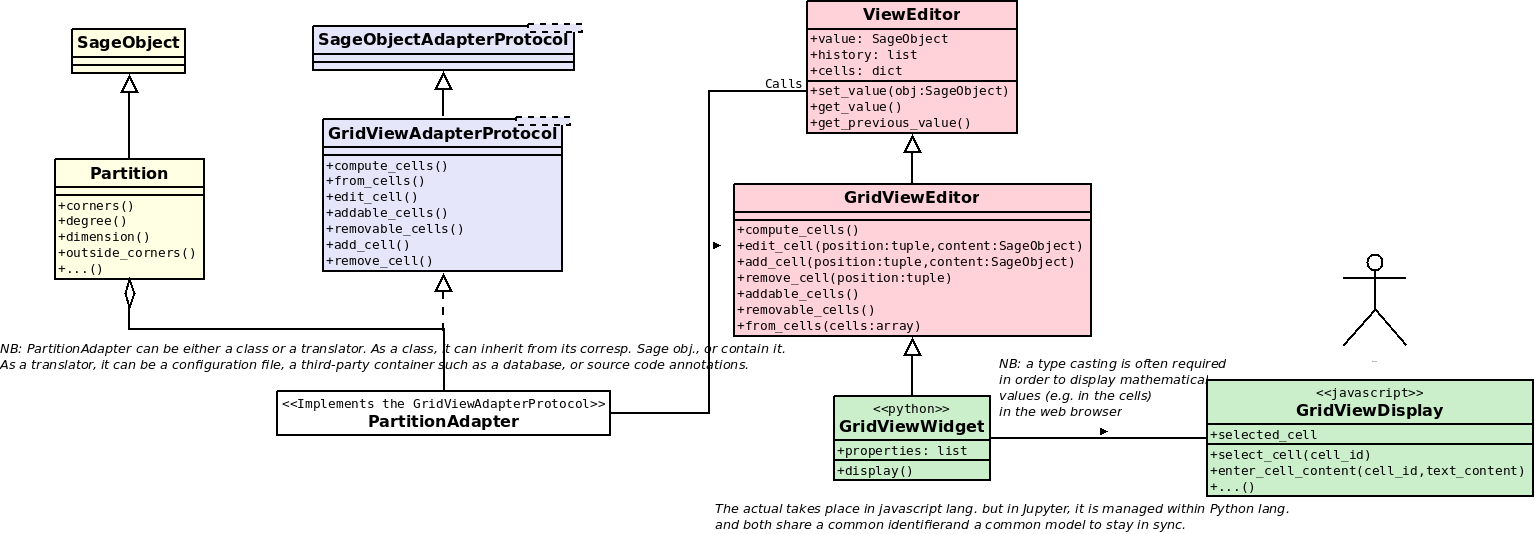
\includegraphics[width=1.4\textheight]{schemas/SageViewEditor}
  \end{center}
  \caption{Sage View Editor classes}
  \label{fig:schema}
\end{figure}
\end{landscape}

\subsection{Dissemination strategy}

The code is distributed as a Sage package
\href{https://github.com/sagemath/sage-combinat-widgets/}{sage-combinat-widgets},
endowed with a Binder-based online demo.
This package is meant to grow beyond this initial seed, attracting
contributions from the community, and presumably be integrated
progressively into SageMath. 

The following steps will be taken to attract users and contributions:
\begin{itemize}
  \item Implementing adapters for the most classical object types, and
    only them;
  \item Writing tutorials on how to write new ones;
  \item Running tutorials at the occasion of local work groups at
    \emph{Laboratoire de Recherche Informatique} and
    \emph{\href{https://www.lix.polytechnique.fr/}{Laboratoire
        d'Informatique de l'École Polytechnique}}, and at upcoming
    Sage Days.
  \item Inviting users to provide feedback, either face to face, on
    the development mailing list, or on the project
    \emph{sage-combinat-widgets} issues interface.
\end{itemize}


% Currently hidden in the \emph{GridViewEditor} itself, we intend to promote
% the development of adapters for the Sage objects, either by implementing Adapter
% classes as such, or by writing translating information. Here are a few code examples
% for both strategies:

% \begin{lstlisting}
% class GenericGraphGridViewAdapter(GenericGraph):
%   ...
%   def from_cells(self, cells={}):
%     g = GenericGraph()
%     g.add_vertices(list(cells.keys()))
%     return g

% class PartitionGridViewAdapter(Partition):
%   ....
%   def add_cell(self, coord):
%     return self.add_cell(self.coord[0], self.coord[1])

% class StandardTableauGridViewAdapter(StandardTableau):
%   ....
%   def from_cells(self, cells={}):
%       positions = sorted(list(cells.keys()))
%       try:
%         return StandardTableau([[cells[pos] for pos in positions if pos[0]==i] for i in uniq([t[0] for t in positions])])
%       except:
%       raise TypeError("Cannot generate a valid StandardTableau!")
% \end{lstlisting}

% Second strategy: a translator can be written directly in the source
% code, with \emph{Python annotations}:

% \begin{lstlisting}
% @grid_view_adapter(\{addable_cells:self.shape().addable_cells, removable_cells:removable_cells\})
% class StandardTableau:
%   /.../
% \end{lstlisting}

%The users can specify their own tile shape. For example they can
%use \emph{IPyWidgets} buttons or text inputs.

%\begin{wrapfigure}{r}{0.25\textwidth}
%    \begin{center}
%      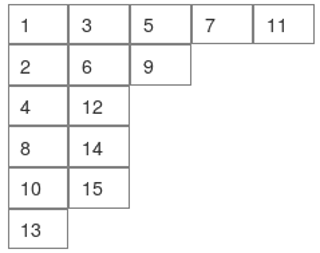
\includegraphics[width=100px]{images/TableauWidget}
%      \caption{A tableau widget}
%\end{center}
%\end{wrapfigure}

\subsection{Future plans}

In the upcoming year, we plan to collaborate tightly with Francy to:
\begin{itemize}
\item Bring Francy's features to \Sage by implementing a backend. This
  would finally bring a solution to a long time yet pressing need of
  the community that was so far only partially fulfilled by
  unsustainable prototypes like Sage's
  \href{http://doc.sagemath.org/html/en/reference/graphs/sage/graphs/graph_editor.html}{graph editor}.
\item Further explore the semantic representation model design pattern
  with over kinds of graphical representations, with a similar
  decoupling between a \Sage backend, a semantic representation model,
  and a Jupyter/JS frontend.
\item Contribute the models and frontends to Francy, making the
  features available to \GAP.
\item Seek collaboration with Macaulay2's
  \href{http://www2.macaulay2.com/Macaulay2/doc/Macaulay2-1.11/share/doc/Macaulay2/Visualize/html/}{Visualize
    package} that share similar aims (though not yet Jupyter based).
\item Write tutorials and collect best practices on how to develop new
  graphical representations on top of Jupyter widgets.
\end{itemize}

\section{Sage-Explorer}
\label{section:sage-explorer}

\subsection{History}

The idea behind Sage-Explorer originated at a workshop organized by
Paul-Olivier Dehaye and the second author at ICMS in 2013. The aim of
this workshop was to bring together developers of online mathematical
databases like the \LMFDB and computational mathematical software like
\Sage.

\LMFDB is an online database in number theory for L-functions and
Modular Forms. One key asset, beyond advanced searches, is the ability
to display objects together with a lot of contextual information, such
as relevant invariants, related objects, and associated mathematical
knowledge; see Figure~\ref{fig:lmfdb-11a2}.
\begin{figure}[h]
  \begin{center}
    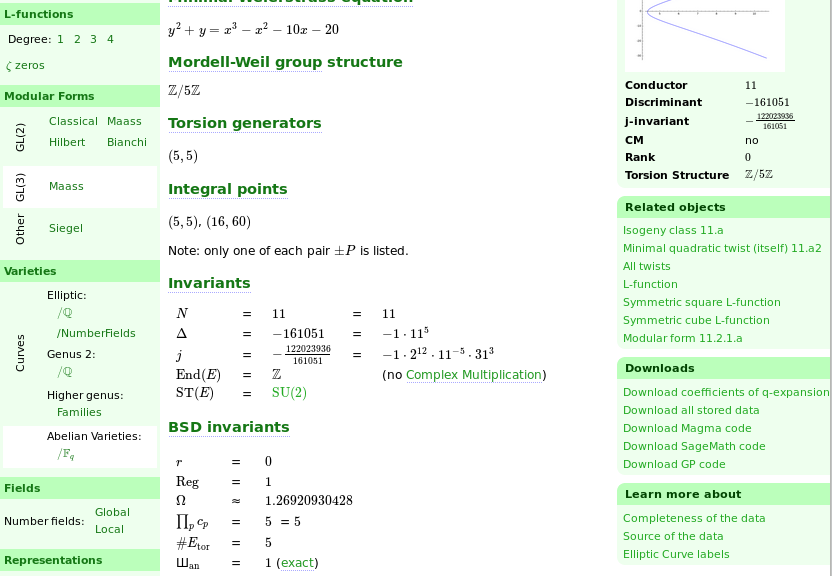
\includegraphics[width=\textwidth]{images/LMFDB-11a2}
  \end{center}
  \caption{The LMFDB page for the elliptic curve ``11a2''.}
  \label{fig:lmfdb-11a2}
\end{figure}
For each type of mathematical object the content of the page is
handpicked by experts, which ensures a highly relevant selection.
However this process does not scale well when the variety of objects
increases. Also, the page can only show precomputed data.

Computational systems like Sage on the other hand let's one compute
with a wide variety of objects; semantic information embedded into the
system makes this scalable by enabling generic code. However, in the
usual Read-Eval-Print loop of a computational system, objects are
displayed without contextual information. Most of the information is
readily available, typically through introspection; however that
introspection needs to be carried out manually which hampers fast pace
interaction and discoverability.

One of many projects at that workshop was to explore whether one could
bridge some of the gap between the two worlds and get the best of
both. Namely, given an object in a computational system, exploiting
the semantic information embedded into the system to generate
automatically a page that displays it together with a relevant
selection of contextual information. Of course, one can't hope to beat
with a generic solution a thoughtful selection made by experts of the
field; nevertheless this may be compensated by the large coverage of
types of objects.

A proof of concept was implemented by Jason Bandlow and the second
author in a matter of days. The implementation was very crude and not
sustainable due to the use of web technologies that did not meld well
with \Sage. Nevertheless, it showed that the concept was meaningful;
more importantly, it led to the discovery that this approach invited
users to go on a journey, exploring \Sage by jumping from objects to
related objects, hence the name, \Sage-Explorer.


\subsection{A \Jupyter-based \Sage-Explorer}

The emergence of the \Jupyter and \Jupyter widget technology at the
time of writing \ODK's proposal opened an opportunity for
reimplementing \Sage-Explorer on top of a sustainable foundation. The
current implementation started in June 2018 and took a few weeks. For
any \Sage object o in a Jupyter session, running \texttt{explore(o)}
opens a page with the following contextual information:
\begin{itemize}
\item a representation of the object, as text, latex formulae,
  graphics, or interactive widget depending on availability;
\item a list of operations (methods) available for the object, sorted
  by the class providing that operation, with the ability to swiftly
  lookup the documentation or run the operation, possibly providing
  additional arguments;
\item a selection of \emph{properties}, that is relevant invariants or
  related objects.
\end{itemize}
See Figure~\ref{fig:sage-explorer-11a2} for the page produced by
Sage-Explorer on the same elliptic curve as above.
\begin{figure}[h]
  \begin{center}
    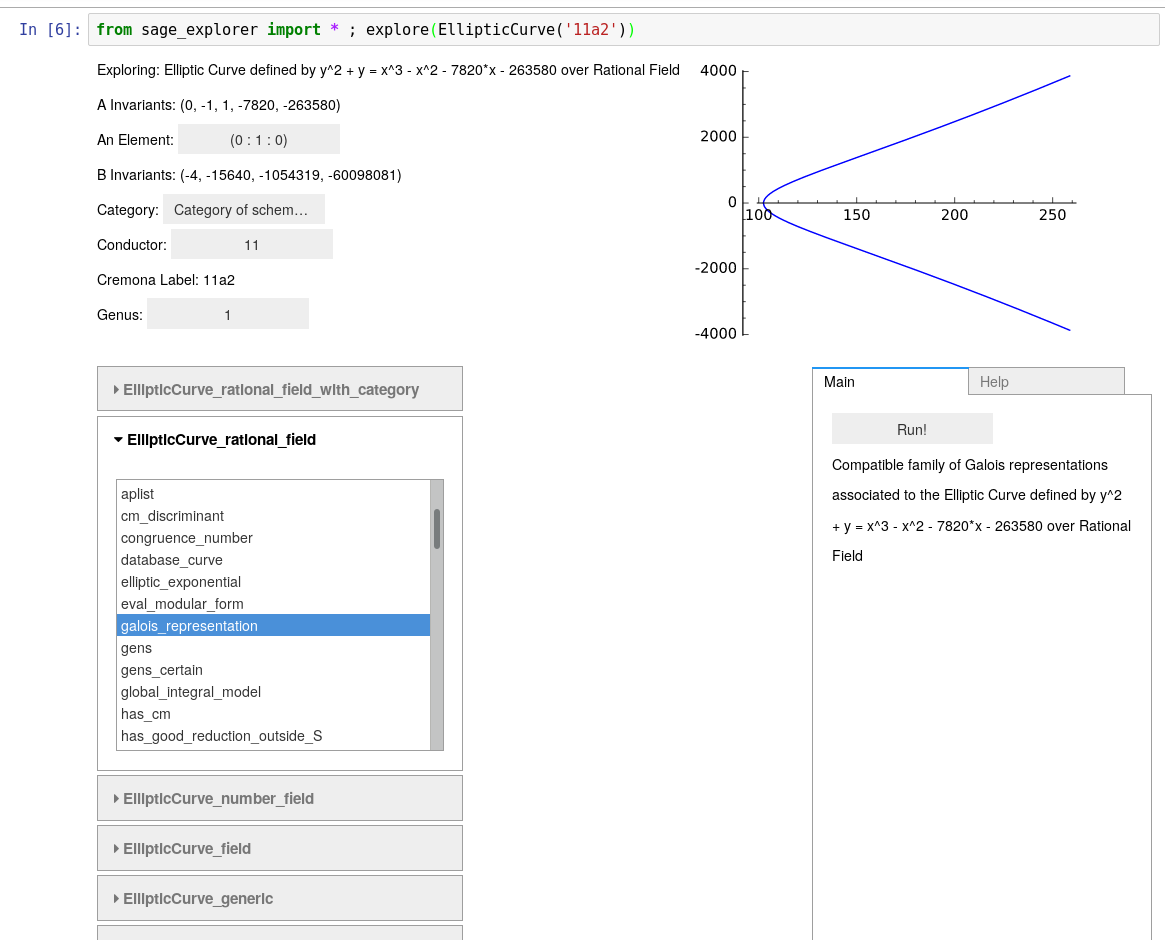
\includegraphics[width=\textwidth]{images/SageExplorer-11a2}
  \end{center}
  \caption{Sage-Explorer on the elliptic curve ``11a2''}
  \label{fig:sage-explorer-11a2}
\end{figure}

% The \href{http://www.lmfdb.org/}{LFMDB} database displays a
% comprehensive view of L-functions and Modular Forms in a web browser,
% yet misses manipulation possibilities on the objects.

% In LMFDB, many methods results are calculated at page opening, while
% with Sage Explorer, the calculation is run only on demand, except for
% some widely used \emph{properties}.

%\TODO{A bunch of screenshots: Tableau? Petersen graph?}

Most objects appearing on the page are clickable to start exploring
them, with history management. The displayed properties are selected
according to the semantic attached to the object. For example, if the
object is a finite set, its cardinality will be displayed. This is
currently configured by a text file in \emph{YAML} syntax a short
extract of which follows.

\ 
\begin{verbatim}

  cardinality:
    in: EnumeratedSets.Finite

  characteristic:
    in: Fields

  genus:
    isinstance: sage.schemes.elliptic_curves.ell_generic.EllipticCurve_generic

  multiplication_table:
    in: Semigroups.Finite
    when: cardinality < 21
\end{verbatim}

Finally, calling \texttt{explore()} without arguments brings up an
index page from which the user can explore Sage's catalogs of graphs,
groups, algebras, crystals, etc.


% The object graphical representations try to be as ``natural'' as
% possible for the user. So we use plotting when relevant. For
% combinatorial objects, we call the \emph{sage-combinat-widgets}
% package. As soon as integration is made with the \emph{sage-combinat-widgets},
% the graphical representation will mirror the object changes in real
% time, too.

% The widget choice is also specified in the configuration. Yet we
% intend to make it available directly within Sage source code, thanks
% to \emph{Python annotations}.

% Sage object methods are listed in the menus to facilite
% discovering, alphabetically ordered. As method lists can be very long,
% we have split them according to the class where they appear in Sage source
% code and we intend to find more than one categorization way.

% When a method is selected, its documentation and signature are made
% available. The user can then fill out the argument and run the method
% to get a result.


% \subsection{Configuration and semantics}
% \label{semantics}

% Three configuration files specify:

% \begin{itemize}
% \item Graphical display widgets associated to Sage objects
%   \item Properties associated to Sage objects, i.e. which object methods are
%     to be considered as object properties.
% \item The objects lists (or \emph{catalogs}) for the Explorer Index
% \end{itemize}

% To specify these, especially the first two, a set of logical rules
% have been defined, are implemented in YAML syntax and parsed by the
% Sage-explorer code.

% In the future, we expect to get all this semantic information, or part of it,
% written directly in Sage source code.

% This could take the form of \emph{private attributes} or \emph{annotations}, like:

% \begin{itemize}
% \item a \emph{\_widget\_} attribute specified in Sage categories source files
% \item specific annotations, using \emph{@} Python syntax for annotations
%   \end{itemize}

% Where will still remain, for the user, the possibility of overloading
% the widget class - \emph{\_widget\_} being only the default) and
% specify which of the \emph{properties} she wants to get rendered in effect.

% Hence, there will be a contiuum between semantic written in Sage
% source code and configuration files, taking into account semantic
% information, logical rules specifying how to read this semantics, and
% parametrization by the user, given that (for \emph{properties}:

% \begin{itemize}
% \item some semantics can be specified as object attributes: ``is this method a
%   property?'' and
%   \item ``is this property worth rendering by default?''  while we
%     still have to decide
%   \item ``is computing this property not going to slow down the display?''
% \end{itemize}

\subsection{Dissemination and future plans}

The code is distributed as a Sage package
\href{https://github.com/sagemath/sage-explorer/}{sage-explorer},
endowed with a Binder-based online demo.

At this stage, Sage-Explorer is still a prototype. It needs to be
battle field tested for stability and usability. We will seek for
feedback from users, in particular for styling, for growing the
properties configuration beyond the current minimal seed, and for
exploring how to best empower them to customize themselves this
configuration. We will also improve the existing features, enabling
for example searches and categorizing of operations, and exploring how
to categorize properties as is done on LMFDB pages.

Last but not least, we will investigate the interplay of Sage-Explorer
with \WPref{dksbases}'s Math-in-the-Middle approach. Recall that this
approach is is to exploit, combine, and enrich the semantic
information contained in computational systems and databases, for
interoperability purposes and beyond. One of the ongoing plans in this
work package is to embed additional semantic information -- like
alignments with the central Math-in-the-Middle ontology -- in \Sage
and other computational systems, for example through code annotations.
Albeit informal, whether a given property is “interesting” for a given
type of objects is semantic information; as such it could be included,
either in the central ontology or in the systems.

We will explore whether the Math-in-the-Middle interoperability layer
can be used to:
\begin{itemize}
\item share the configuration of interesting properties?
\item explore other other computational systems from Sage?
\item derive native explorers for other systems with minimal custom
  code for each system?
\end{itemize}

% \subsection{Strategy to get feedback from users?}

% \TODO{See above (ou bien on recopie dès que c'est bien fixé)}

% \appendix

% \TODO{The demo notebooks?}

\end{document}

%%% Local Variables:
%%% mode: latex
%%% TeX-master: t
%%% End:
